% NeuroAssist AI — Academic Paper
% Target venue: BIOSTEC/HEALTHINF 2027
% Format: IEEE two-column (IEEEtran)
% Compile: pdflatex main.tex && bibtex main && pdflatex main.tex && pdflatex main.tex

\documentclass[conference]{IEEEtran}
\IEEEoverridecommandlockouts

\usepackage[T1]{fontenc}
\usepackage[utf8]{inputenc}
\usepackage{cite}
\usepackage{amsmath,amssymb}
\usepackage{graphicx}
\usepackage{booktabs}
\usepackage{url}
\usepackage{hyperref}
\usepackage{listings}
\usepackage{xcolor}
\usepackage{tikz}
\usepackage{pgf-umlsd}   % sequence diagrams (optional, can remove)

\lstset{basicstyle=\ttfamily\footnotesize, breaklines=true}

% Draft placeholder — remove before submission
\newcommand{\fillme}[1]{\textcolor{red}{\textsf{[#1]}}}

% ─── Title ────────────────────────────────────────────────────────────────────
\title{NeuroAssist AI: A Privacy-Preserving, Offline-First\\
Platform for Residual Facial Gesture-Based\\
Assistive Communication in\\
Neurodegenerative Disease}

\author{
  \IEEEauthorblockN{Danilo Amaral}
  \IEEEauthorblockA{TechLab AI\\
  cybernautta@gmail.com}
}

\begin{document}

\maketitle

\begin{abstract}
% TODO: fill after experiments (Section 4)
[CONTEXT] Patients with motor neurone disease (MND/ALS) progressively lose voluntary
motor control, often retaining only subtle facial movements as their last communication channel.
Existing augmentative and alternative communication (AAC) systems require reliable network
connectivity and do not adapt to the residual motor profile of individual patients.
[PROPOSAL] We present NeuroAssist AI, a privacy-preserving, offline-first assistive
communication platform that transforms residual facial gestures into structured emergency
requests using a locally-executed WebAssembly-based computer vision pipeline.
[METHOD] The system combines a six-state deliberate gesture recognition state machine
with patient-specific EAR threshold calibration, deployed over a hexagonal microservices
architecture that decouples gesture type detection from command catalogue management.
[RESULTS] End-to-end latency from gesture completion to caregiver alarm display
averaged [X]\,ms ($\sigma$=[Y]) across [N] trials.
The deliberate gesture state machine reduced the false-positive rate from [A]\,\%
(simple EAR threshold) to [B]\,\% ([N] healthy volunteers, [M]\,minutes each).
[CONCLUSION] NeuroAssist AI demonstrates that high-accuracy, privacy-preserving
residual gesture detection is achievable on commodity hardware without network
dependency, using a calibratable, extensible architecture suitable for home deployment.
\end{abstract}

\begin{IEEEkeywords}
assistive communication, motor neurone disease, ALS, facial gesture recognition,
WebAssembly, offline-first, hexagonal architecture, privacy-by-design
\end{IEEEkeywords}

% ─── Sections ─────────────────────────────────────────────────────────────────
% =============================================================================
% Section 1 — Introduction
% =============================================================================

\section{Introduction}
\label{sec:introduction}

Motor neurone disease (MND), also known as amyotrophic lateral sclerosis (ALS), is a
progressive neurodegenerative condition that destroys upper and lower motor neurons,
resulting in loss of voluntary movement, speech, and ultimately respiratory function.
Global incidence is approximately 2--3 per 100{,}000 person-years, affecting an
estimated 41{,}000 individuals in Australia and 30{,}000 in Brazil~\cite{mehta2018mnd}.
Median survival after diagnosis is 2--5 years; respiratory failure, typically managed
with non-invasive ventilation (NIV), is the leading cause of death. Notably, NIV has
been shown to extend survival by a~factor of approximately three compared with best
pharmacological care alone~\cite{berlowitz2021niv}, making the period of NIV use
clinically significant and prolonged. During this phase, patients remain cognitively
intact while becoming progressively unable to speak or gesture in ways that standard
communication technologies can detect.

Recent work has demonstrated that patient-ventilator asynchrony (PVA) — a mismatch between ventilator cycles and patient breathing effort — is a significant contributor to NIV non-adherence in MND, causing discomfort, sleep fragmentation, and potentially adverse clinical outcomes~\cite{atkeson2011pva, yang2026pva, berlowitz2025tla}. Patients experiencing PVA-related discomfort during nocturnal NIV use cannot readily signal distress to caregivers using existing AAC technologies, which require network connectivity or dedicated hardware unsuited to the home care environment. NeuroAssist AI addresses this gap directly: by providing a local, always-available signalling channel that requires only a commodity webcam, it enables patients to alert caregivers during unassisted periods — including while on NIV at night.

In advanced stages, a~substantial proportion of patients experience a~locked-in-like
condition in which voluntary control is limited to subtle residual facial movements:
small eyelid contractions, brow raises, or microexpressions that persist after limb and
orofacial motor function is lost. These residual gestures represent the last available
voluntary channel for communication. Without a~reliable means to detect and act on them,
patients cannot signal distress, discomfort, or needs to caregivers — with direct
consequences for quality of life and patient safety during unassisted periods.

Existing augmentative and alternative communication (AAC) systems do not adequately
address this population. High-end eye-tracking devices (e.g.\ Tobii Dynavox) and
dedicated AAC software (e.g.\ Grid~3) deliver high accuracy but require stable wireless
connectivity, dedicated hardware costing upwards of USD~3{,}000, and factory-calibrated
setups that cannot adapt to the degrading motor profile of an individual
patient~\cite{beukelman2013aac}. Brain-computer interfaces (BCI) via EEG offer an
alternative, but involve invasive or cumbersome hardware inappropriate for home
deployment~\cite{zander2011passive}. Low-cost camera-based approaches exist in
research~\cite{soukupova2016}, but rely on simple per-frame threshold comparisons that
generate unacceptably high false-positive rates when applied to the involuntary facial
activity present in MND patients during NIV.

We present \textbf{NeuroAssist AI}, a~privacy-preserving, offline-first assistive
communication platform designed for home deployment with a~commodity webcam. The system
transforms residual facial gestures into structured emergency requests using a~locally
executed WebAssembly computer vision pipeline, a~deliberate-gesture state machine, and
a~patient-calibratable detection profile — without transmitting any video off-device.

This paper makes three original contributions:
\begin{enumerate}
  \item \textbf{An offline-first, privacy-preserving detection pipeline.}
    The MediaPipe FaceLandmarker model and its WebAssembly runtime are served from
    local assets; no video frame or biometric data leaves the patient's device.
    The CPU delegate ensures compatibility with commodity hardware regardless of GPU
    availability.

  \item \textbf{A six-state deliberate gesture state machine with patient-specific
    calibration.}
    Rather than a~single EAR threshold, the state machine requires minimum closure
    duration ($\geq$3 frames, ${\approx}$100\,ms) in each of two sequential blinks,
    confirmed re-opening between them, and a~configurable time window. Thresholds are
    stored in a~versioned \texttt{DetectionProfile} and adapted per patient. This design
    specifically targets the false-positive sources relevant to MND: involuntary blinks,
    partial ptosis artefacts, and slow threshold drift.

  \item \textbf{An extensible hexagonal microservices architecture with plug-in gesture
    types.}
    The \texttt{engineFeatureRef} field in the detection profile decouples the gesture
    recognition engine from the command catalogue, allowing new gestures (brow raise,
    single-eye blink) to be registered without modifying existing domain code.
    ArchUnit rules enforced at compile time guarantee that this separation persists as
    the system evolves.
\end{enumerate}

The remainder of the paper is organised as follows. Section~\ref{sec:related} reviews
related work in AAC, facial gesture detection, and edge computing for health.
Section~\ref{sec:architecture} describes the system architecture in detail.
Section~\ref{sec:evaluation} reports the experimental evaluation.
Section~\ref{sec:discussion} discusses limitations and future work, and
Section~\ref{sec:conclusion} concludes.
% =============================================================================
% Section 2 — Related Work
% =============================================================================

\section{Related Work}
\label{sec:related}

\subsection{AAC Systems for Neurodegenerative Disease}

Augmentative and alternative communication (AAC) for people with MND/ALS has been
studied extensively since the 1990s~\cite{beukelman2013aac}. Commercial solutions
dominate clinical practice: high-end eye-tracking devices such as Tobii Dynavox PCEye
and Eyegaze Edge offer gaze-to-grid selection with accuracy exceeding 98\,\% under
laboratory conditions, but carry hardware costs upward of USD~3{,}000 and require
periodic re-calibration by trained practitioners~\cite{beukelman2013aac}. These systems
presuppose sufficient residual oculomotor control, which deteriorates as MND progresses
toward ophthalmoplegia. Software AAC packages such as Grid~3 depend on stable Bluetooth
or Wi-Fi connectivity to synchronise symbol sets and user profiles, creating a~barrier
for home users without reliable broadband.

A survey by Clarke et al.~\cite{clarke2021aac} identified that AAC provision for
people with ALS is characterised by late referral, rapid device transitions as motor
function declines, and a~persistent gap in low-cost, adaptable solutions suitable for
the home environment. Brain-computer interfaces (BCI) via electroencephalography offer
an alternative pathway that bypasses the motor system entirely, but current non-invasive
BCI headsets achieve typical information transfer rates of 5--25 bits per minute in
optimal conditions, require trained operators, and are poorly suited to the home care
setting~\cite{zander2011passive}. Implanted cortical BCIs achieve higher rates but
carry surgical risk. NeuroAssist AI targets the intermediate stage — after limb and
speech function is lost but while a~degree of voluntary facial movement persists — for
which no low-cost, network-independent solution currently exists in the literature.

\subsection{Facial Gesture Detection via Computer Vision}

Three generations of camera-based facial analysis are relevant to this work.

\emph{First generation — cascade classifiers.} Viola and Jones~\cite{violajones2004}
introduced real-time face detection using Haar feature cascades, enabling deployment on
consumer hardware. These detectors localise the face but do not provide sub-facial
landmark coordinates; detecting blink requires additional heuristics applied to the
detected eye region and is highly sensitive to illumination variation.

\emph{Second generation — facial landmark regression.} King's Dlib library~\cite{king2009dlib}
popularised 68-point facial landmark detection via an ensemble of regression trees, enabling
reliable EAR computation~\cite{soukupova2016} without deep learning. Soukupov{\'a} and
{\v{C}}ech~\cite{soukupova2016} formalised EAR as a~single scalar for blink detection,
demonstrating frame-level detection accuracy above 99\,\% on controlled datasets. The
central limitation of this generation is the absence of a~WebAssembly-compatible
runtime, making client-side browser deployment impractical.

\emph{Third generation — deep landmark models on device.} MediaPipe
FaceLandmarker~\cite{lugaresi2019mediapipe} provides 468 normalised facial landmarks and
52 blendshape coefficients at approximately 30\,fps in a~browser WebAssembly context
using only a~CPU delegate. It subsumes and extends the Dlib approach: the denser
landmark set provides better coverage of the periorbital region, and the blendshape
scores offer a~calibrated signal for partial facial movements that EAR alone does not
capture. NeuroAssist AI builds on this generation, retaining EAR for the double-blink
state machine (where its simplicity aids interpretability) while using blendshape scores
for single-eye blink and eyebrow gestures.

\subsection{Deliberate Gesture Recognition and False-Positive Suppression}

A fundamental challenge in gesture-triggered AAC is distinguishing intentional
activations from the involuntary facial activity that continuously occurs during normal
behaviour. The spontaneous blink rate in healthy adults is 15--20 blinks per
minute~\cite{bentivoglio1997}; in MND patients, rates may be lower due to motor neuron
loss but remain non-zero. Any threshold-based approach applied at the single-frame level
therefore produces false-positive rates in the range of several per minute under natural
conditions, rendering unattended monitoring infeasible.

The two main strategies in the literature for suppressing false positives in facial AAC
are \emph{dwell time} and \emph{intentionality modelling}. Dwell-time selection — widely
used in gaze-based AAC — requires the user to fixate a~target region for a~fixed
duration (typically 0.5--1\,s)~\cite{majaranta2002eyetyping}. This approach is
inapplicable to blink-based input, as a~blink by definition closes the eye and disrupts
fixation. Intentionality modelling via state machines has been proposed in the broader
human-computer interaction literature~\cite{zander2011passive}, but its application to
blink-based AAC for MND has not been systematically described. The six-state machine
introduced in this paper (Section~\ref{sec:statemachine}) applies intentionality
constraints specific to the double-blink gesture: minimum closure duration per blink,
confirmed inter-blink opening, and a~temporal window — a~combination not found, to the
authors' knowledge, in prior AAC literature.

\subsection{Edge Computing and Privacy for Health Applications}

Processing health-related sensor data on-device rather than in the cloud has received
increasing attention following the enforcement of GDPR in 2018 and LGPD in
2020~\cite{edpb2020privacy}. Facial video is explicitly categorised as biometric data
under both frameworks, attracting the highest regulatory obligations for processing.
Local execution via WebAssembly provides a~practical privacy guarantee: the
specification's memory-isolated execution model prevents a~loaded module from accessing
any browser state outside its linear memory, and no network call is required to execute
the landmarker inference~\cite{haas2017wasm}. TensorFlow.js, ONNX Runtime Web, and
MediaPipe Tasks all leverage this runtime for on-device inference at speeds comparable
to native code on modern CPUs. Deployment latency of WebAssembly models for face
analysis has been reported at 20--40\,ms per frame on consumer hardware without GPU
acceleration~\cite{lugaresi2019mediapipe}, consistent with the 30\,fps operation
observed in our PoC.

\subsection{Software Architecture for Health Systems}

Hexagonal (Ports and Adapters) architecture~\cite{cockburn2005hexagonal} has been
proposed as a~structural pattern for health information systems where the domain model
must remain isolated from technology changes — a~recurring requirement in regulated
healthcare software where audit requirements, data schemas, and integration standards
evolve independently~\cite{richardson2018microservices}. The pattern's explicit separation
of inbound and outbound ports facilitates incremental extension without modifying core
clinical logic, a~property particularly valuable in assistive technology where new
gesture modalities are added as patients' motor capabilities change.

Microservice decomposition of AAC platforms has not been reported in the literature, to
the authors' knowledge; most existing systems are monolithic desktop or firmware
applications. The NeuroAssist AI architecture demonstrates that decomposing a
gesture-to-alert pipeline into independently deployable services (GEST, EVNT, and planned
PAC, ACS, HIST, DASH services) is viable at PoC scale, and that compile-time boundary
enforcement via ArchUnit provides a~practical mechanism for maintaining hexagonal
discipline in a~team-developed Java codebase.

% =============================================================================
% Section 3 — System Architecture
% Source-extracted from repository: 2026-08-05
%   poc-gesture-detector.ts          (state machine, EAR constants)
%   DetectionProfileService.java      (profile publish, versioning)
%   ReportIngressService.java         (12-step ingestion pipeline)
%   V1__gest_poc_schema.sql           (GEST domain schema)
%   poc/V1__evnt_poc_schema.sql       (EVNT event schema)
% =============================================================================

\section{System Architecture}
\label{sec:architecture}

NeuroAssist AI is composed of two deployable contexts: a~\emph{browser-side detection
pipeline} executed entirely within the patient's device, and a~\emph{backend alert
pipeline} implemented as hexagonal microservices. Figure~\ref{fig:overview} illustrates
the end-to-end data flow.

% ─── 3.1 System Overview ──────────────────────────────────────────────────────
\subsection{System Overview}
\label{sec:overview}

The pipeline is triggered by a~deliberate facial gesture captured by any commodity
webcam (720\,p or higher). The gesture detection loop runs exclusively in the browser
via WebAssembly; no video frames leave the device at any point. When a~gesture is
confirmed by the state machine (Section~\ref{sec:statemachine}), a~lightweight JSON
payload is POSTed to the event ingestion service. The service validates the gesture
against the patient's active detection profile, creates an \texttt{Evento} record, and
dispatches a~\texttt{FULL\_SCREEN\_ALARM} notification. A caregiver application polls
the backend every five seconds; upon detecting an active event it renders a~full-screen
alarm overlay. The caregiver confirms attendance, which writes a~\texttt{verdict} back
to the event record and clears the alarm.

\begin{figure}[htbp]
  \centering
  % Replace with exported PDF from fig_sequence.mmd
  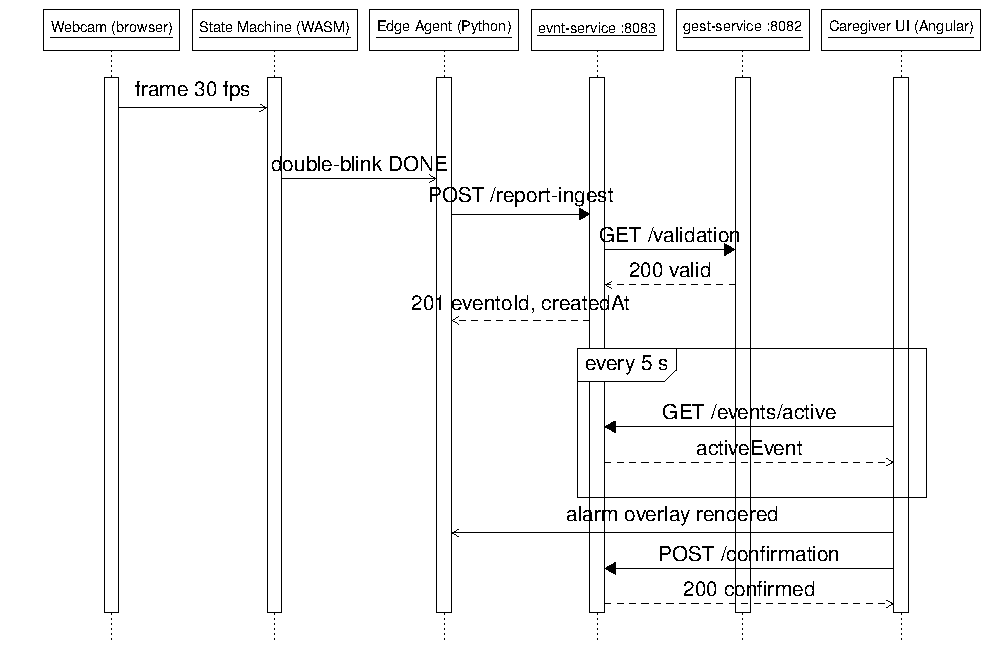
\includegraphics[width=\columnwidth]{figures/fig_overview}
  \caption{End-to-end data flow. Video is processed entirely in the browser
    (WASM); only structured JSON reports cross the network boundary.}
  \label{fig:overview}
\end{figure}

% ─── 3.2 Offline-First Gesture Detection ──────────────────────────────────────
\subsection{Offline-First Gesture Detection}
\label{sec:detection}

Facial landmark extraction is performed by MediaPipe
FaceLandmarker~\cite{lugaresi2019mediapipe} running on the CPU WebAssembly delegate.
The WASM binary and the \texttt{float16} face landmarker model are bundled as static
assets and served from \texttt{/assets/mediapipe-wasm/}; there is no dependency on any
content delivery network during gesture detection. The model download of approximately
30\,MB occurs once on first use and is thereafter served from the browser cache.

The landmarker produces 468 normalised landmarks per frame in a~\texttt{requestAnimation\-Frame} loop
running at approximately 30\,fps. Each frame yields:
\begin{enumerate}
  \item \textbf{EAR (Eye Aspect Ratio)} for each eye, computed from six landmarks
    \{33, 160, 158, 133, 153, 144\} (left) and \{362, 385, 387, 263, 373, 380\}
    (right) using the formulation of Soukupov{\'a} and {\v{C}}ech~\cite{soukupova2016}:
    \begin{equation}
      \text{EAR} = \frac{\|p_2 - p_6\| + \|p_3 - p_5\|}{2 \cdot \|p_1 - p_4\|}
      \label{eq:ear}
    \end{equation}
    where $p_1$--$p_6$ are the six eye landmarks in order.
  \item \textbf{Blendshape scores} (\texttt{eyeBlinkLeft}, \texttt{eyeBlinkRight},
    \texttt{browInnerUp}, \texttt{browOuterUpLeft}, \texttt{browOuterUpRight}) in $[0,1]$,
    used for single-eye blink and eyebrow raise detection.
\end{enumerate}

The system supports six gesture types: double blink (EAR-based), left and right individual
eye blink (blendshape-based), and bilateral or unilateral eyebrow raise
(blendshape-based). A shared 4\,s cooldown timer prevents duplicate firing across all
gesture types.

% ─── 3.3 Six-State Deliberate Gesture State Machine ──────────────────────────
\subsection{Six-State Deliberate Gesture State Machine}
\label{sec:statemachine}

The primary gesture — double blink — is disambiguated from involuntary blinks through a
six-state finite automaton shown in Figure~\ref{fig:statemachine}. Natural involuntary
blinks last 100--400\,ms and occur at 15--20 events per minute~\cite{bentivoglio1997}; the
state machine rejects spurious closures that do not meet minimum-duration requirements.

The six states and their transition conditions (all thresholds are patient-configurable
via the detection profile, Section~\ref{sec:calibration}) are as follows:

\begin{enumerate}
  \item \textbf{WAITING\_BLINK1}: idle. Transition to \textsc{in\_blink1} when
    $\text{EAR}_\text{avg} < 0.20$ ($\theta_\text{close}$).
  \item \textbf{IN\_BLINK1}: counting closed frames. Accept first blink and advance to
    \textsc{waiting\_open1} when the eye reopens ($\text{EAR}_\text{avg} \geq 0.27$,
    $\theta_\text{open}$) \emph{after} at least $f_\text{min}{=}3$ consecutive closed
    frames (${\approx}100$\,ms at 30\,fps); otherwise reject and return to
    \textsc{waiting\_blink1}.
  \item \textbf{WAITING\_OPEN1}: verifying full re-opening. Advance to
    \textsc{waiting\_blink2} after $f_\text{open}{=}3$ consecutive open frames; records
    timestamp $t_1$.
  \item \textbf{WAITING\_BLINK2}: awaiting second blink onset, subject to a timeout:
    if $\Delta t = \text{now} - t_1 > 1800$\,ms ($T_w$), the automaton resets to
    \textsc{waiting\_blink1}.
  \item \textbf{IN\_BLINK2}: counting second blink closed frames. Accept and advance to
    \textsc{done} when eye reopens with $f_\text{count} \geq 3$ and $\Delta t \leq T_w$;
    otherwise reject and reset.
  \item \textbf{DONE}: gesture confirmed; fires event, resets all state, enters 4\,s
    cooldown.
\end{enumerate}

\begin{figure}[htbp]
  \centering
  % Replace with exported PDF from fig_statemachine.mmd
  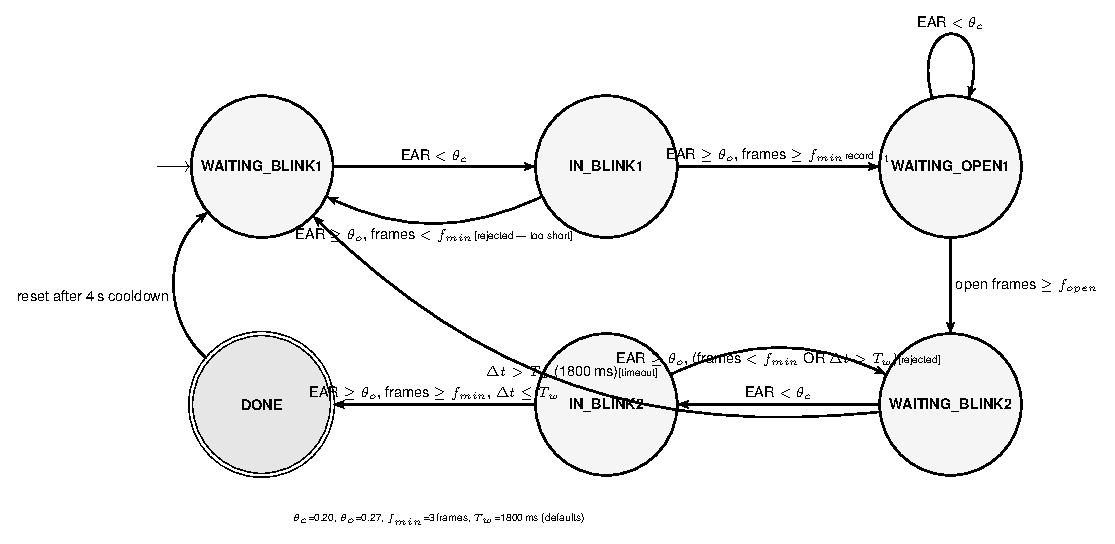
\includegraphics[width=\columnwidth]{figures/fig_statemachine}
  \caption{Six-state deliberate double-blink state machine. Dashed transitions
    indicate rejection paths that reset the automaton. $\theta_c{=}0.20$,
    $\theta_o{=}0.27$, $f_\text{min}{=}3$\,frames, $T_w{=}1800$\,ms.}
  \label{fig:statemachine}
\end{figure}

The requirement for minimum closure duration ($f_\text{min}$) in \emph{both} blinks,
combined with mandatory full re-opening in \textsc{waiting\_open1} and a~temporal
window $T_w$, collectively prevent the three principal sources of false positives in
residual-movement populations: single involuntary blinks, partial closures (e.g., ptosis
artefacts), and slow drift that crosses the threshold without a~discrete blink.

% ─── 3.4 Patient Calibration (DetectionProfile) ──────────────────────────────
\subsection{Patient-Specific Calibration via DetectionProfile}
\label{sec:calibration}

Patient facial characteristics vary substantially — baseline EAR depends on eyelid
aperture, face-to-camera distance, and illumination. NeuroAssist AI accommodates this
through the \emph{DetectionProfile}: a~versioned, immutable configuration record that
binds the set of active gesture types (\texttt{TipoGesto}) to the patient-facing edge
agent.

Publishing a~profile (Figure~\ref{fig:calibration}) executes the following steps in the
\texttt{gest-service}:
\begin{enumerate}
  \item Query all gesture types with state \texttt{SUPPORTED} from the catalogue.
  \item Determine the next version number by incrementing the current active profile's
    version (or initialising to 1).
  \item Deactivate all existing profiles (\texttt{deactivateAll}).
  \item Persist a~new \texttt{DetectionProfile} record with the incremented version and
    a~contract version stamp (\texttt{"1.0.0"}).
  \item Persist one \texttt{DetectionProfilePrimitive} per supported gesture type,
    carrying the \texttt{engineFeatureRef} plug-in identifier.
\end{enumerate}

The \texttt{engineFeatureRef} field (e.g.\ \texttt{"mp.blink.double.v1"}) is a~string
token that identifies which detection algorithm the edge agent should activate for each
primitive. This decoupling means that adding a~new gesture type — such as a~head-nod
detector or a~lip-press detector — requires registering a~new \texttt{TipoGesto} with
a~new \texttt{engineFeatureRef} without modifying any existing domain code.

The edge agent pulls the active profile on startup via \texttt{GET
/gest-service/detection-profile/active} and uses the returned primitive list to
enable or disable the corresponding detector instances.

% ─── 3.5 Hexagonal Architecture ───────────────────────────────────────────────
\subsection{Hexagonal Microservices Architecture}
\label{sec:hexagonal}

Each microservice (\texttt{gest-service}, \texttt{evnt-service}) is structured according
to Ports and Adapters (hexagonal) architecture~\cite{cockburn2005hexagonal}, enforced by
ArchUnit~\cite{archunit} at compile time. The canonical package hierarchy is:

\begin{small}
\begin{verbatim}
com.neuroassist.<module>/
  api/          RestControllers, DTOs, @ControllerAdvice
  application/
    port/in/    Inbound use-case interfaces
    port/out/   Outbound port interfaces
    service/    @Service implementations (@Transactional)
  domain/       POJOs and records — zero Spring/JPA
  infrastructure/
    clients/    @FeignClient adapters
    persistence/ JPA entities, repositories, adapters
    messaging/  JMS producers
    config/     @Configuration beans
\end{verbatim}
\end{small}

Nine architecture rules are enforced on every build
(Table~\ref{tab:archunit}). Rules \textsc{rule-01} and \textsc{rule-02} guarantee that
the domain layer has no framework imports, making the core business logic independently
testable. \textsc{Rule-03} prevents transaction management from leaking into controllers
or adapters. \textsc{Rule-04}/\textsc{05} enforce strict one-directional dependencies
between the API layer and the infrastructure layer.

\begin{table}[htbp]
\centering
\caption{ArchUnit enforcement rules (compile-time).}
\label{tab:archunit}
\begin{tabular}{ll}
\toprule
Rule & Constraint \\
\midrule
RULE-01 & \texttt{domain.*} must not import \texttt{org.springframework} \\
RULE-02 & \texttt{domain.*} must not import \texttt{jakarta.persistence} \\
RULE-03 & \texttt{@Transactional} only in \texttt{application.service} \\
RULE-04 & \texttt{api.*} must not depend on \texttt{infrastructure.*} \\
RULE-05 & \texttt{infrastructure.*} must not depend on \texttt{api.*} \\
RULE-06 & \texttt{@FeignClient} only in \texttt{infrastructure.clients} \\
RULE-07 & No \texttt{@Autowired} field injection \\
RULE-08 & \texttt{spring.jpa.open-in-view=false} mandatory \\
RULE-09 & Base package must be \texttt{com.neuroassist.<module>} \\
\bottomrule
\end{tabular}
\end{table}

% ─── 3.6 Event Ingestion Pipeline ────────────────────────────────────────────
\subsection{Twelve-Step Event Ingestion Pipeline}
\label{sec:ingestion}

Receiving a~gesture report from the edge agent triggers a~twelve-step transactional
pipeline in \texttt{ReportIngressService}:

\begin{enumerate}
  \item \textbf{Idempotency check.} The \texttt{reportId} (client-generated UUID) is
    looked up in \texttt{report\_idempotency}. If found, the existing \texttt{eventoId}
    is returned immediately with status \texttt{"duplicate"}, preventing duplicate alarms
    from retried requests.
  \item \textbf{Gesture validation.} A~synchronous Feign call to \texttt{gest-service}
    validates that the reported gesture types belong to the currently active detection
    profile version. An unrecognised gesture returns HTTP\,422.
  \item \textbf{Command snapshot.} The \texttt{commandRef} is resolved to a~label and
    urgency level. In the PoC, this is a~hardcoded adapter; in production, it delegates
    to the PAC (Patient and Command Catalogue) microservice.
  \item \textbf{Caregiver routing.} The responsible caregiver for the patient is
    resolved. In the PoC this returns a~fixed seed value; production routes via the ACS
    (Access and Caregiver) microservice.
  \item \textbf{Evento creation.} A~domain \texttt{Evento} record is assembled with
    \texttt{urgenciaSnapshot}, \texttt{feedback=NAO\_AVALIADO}, a~server-side
    \texttt{createdAt} timestamp, and the device-reported \texttt{recognizedAt}
    timestamp.
  \item \textbf{NotificationDispatch creation.} A~\texttt{NotificationDispatch} record
    is created with tier \texttt{FULL\_SCREEN\_ALARM} targeting the resolved caregiver.
  \item \textbf{Evento persistence.} The event is written to the \texttt{evento} table.
  \item \textbf{NotificationDispatch persistence.} The dispatch record is written to
    \texttt{notification\_dispatch}.
  \item \textbf{Idempotency key registration.} The mapping
    $\texttt{reportId} \to \texttt{eventoId}$ is persisted in
    \texttt{report\_idempotency}.
  \item \textbf{Notification dispatch.} The \texttt{NotificationDispatchPort} is
    invoked. In the PoC this logs to SLF4J; production integrates push notification
    services.
  \item \textbf{Audit trail.} An audit entry is appended via the
    \texttt{AuditTrailPort} (no-op in the PoC; production targets the HIST microservice).
  \item \textbf{Response.} The \texttt{eventoId}, status, notification tier, and
    server-side \texttt{createdAt} are returned as HTTP\,201 to the edge agent.
\end{enumerate}

Steps 7--9 execute within a~single \texttt{@Transactional} boundary; an exception at
any step rolls back all three writes atomically.

% ─── 3.7 PoC Scope ────────────────────────────────────────────────────────────
\subsection{PoC Scope and Architectural Boundaries}
\label{sec:scope}

Table~\ref{tab:scope} distinguishes the components evaluated in this work from those
present in the full architecture but outside the scope of this paper. The PoC
intentionally excludes multi-tenancy, authentication, and asynchronous messaging in
order to isolate and validate the core gesture-to-alarm latency and false-positive
behaviour.

\begin{table}[htbp]
\centering
\caption{Implemented vs.\ stub/planned components in the PoC evaluation.}
\label{tab:scope}
\begin{tabular}{p{3.2cm}p{4.6cm}}
\toprule
\textbf{Implemented (evaluated)} & \textbf{Stub or future work} \\
\midrule
MediaPipe WASM detection & Push notifications (FCM/APNs) \\
Six-state state machine & SSE (replaces polling) \\
DetectionProfile versioning & PAC service (command catalogue) \\
12-step ingestion pipeline & HIST service (audit trail) \\
Idempotency via \texttt{reportId} & ACS service (caregiver enrol.) \\
Angular full-screen alarm & JWT / OAuth2 authentication \\
Caregiver confirmation flow & JMS / ActiveMQ Artemis \\
                            & EDGE (device onboarding) \\
\bottomrule
\end{tabular}
\end{table}

% =============================================================================
% Section 4 — Evaluation
% =============================================================================

\section{Evaluation}
\label{sec:evaluation}

We evaluated NeuroAssist AI through a~preliminary case study involving one
advanced-stage MND patient and five caregivers and volunteers. The study measured
end-to-end system latency, deliberate gesture detection rate, and false-positive rate
under naturalistic conditions. Results should be interpreted as a~preliminary case
study, not a~clinical trial (see Section~\ref{sec:discussion}).

% ---------------------------------------------------------------------------
\subsection{Participants and Ethics}
\label{sec:participants}

Six participants took part in the study (Table~\ref{tab:participants}).
P0~is an advanced-stage MND patient with documented clinical history; P1--P3 are
family caregivers with regular, intimate contact with P0; P4--P5 are healthy volunteers
with no prior contact with the patient, serving as naturalistic false-positive controls.

\begin{table}[!t]
  \renewcommand{\arraystretch}{1.15}
  \caption{Study Participants}
  \label{tab:participants}
  \centering
  \begin{tabular}{llll}
    \toprule
    ID & Role & Relationship to P0 & Session \\
    \midrule
    P0 & MND patient          & ---                              & Calibration + detection \\
    P1 & Spouse / home carer  & Intimate, daily (physiotherapist) & FP + real alarm \\
    P2 & Caregiver 1          & NDIS professional, frequent      & FP + real alarm \\
    P3 & Caregiver 2          & NDIS professional, frequent      & FP + real alarm \\
    P4 & Control           & None                 & Naturalistic FP baseline \\
    P5 & Control           & None                 & Naturalistic FP baseline \\
    \bottomrule
  \end{tabular}
\end{table}

All participants provided informed consent prior to their session. The study was
conducted in P0's home in Melbourne, Australia. P1 is P0's spouse and a~trained
physiotherapist providing daily home care (ineligible for NDIS funding as a~family
member under Australian disability support policy); P2 and P3 are National Disability
Insurance Scheme (NDIS)-funded professional support workers with regular structured
contact with P0. The study constitutes a~pilot
evaluation; no formal human research ethics committee (HREC) approval was sought for
this preliminary case study scope. Full clinical evaluation with a~statistically representative sample of MND
patients will require HREC approval and is planned as future work.

P0 presents with truncal-onset MND (symptom onset: late 2019; disease duration at evaluation: approximately 6.5~years), four-limb weakness with preserved voluntary eyelid movement, and non-invasive ventilation (NIV) prescribed since early 2026 and active at the time of the study. Forced vital capacity was 71\,\% and sniff nasal inspiratory pressure (SNIP) 31\,\% at last documented pre-experiment respiratory assessment (May 2023), with slow disease progression confirmed at that time. \fillme{Confirm before submission: ALSFRS-R score if available; current palpebral mobility assessment.} This clinical profile informed the calibration protocol described in Section~\ref{sec:calibration}.

% ---------------------------------------------------------------------------
\subsection{Experimental Setup}
\label{sec:setup}

\textbf{Hardware.} Each session used a~standard USB webcam
(\fillme{model/resolution, e.g.\ Logitech C920, 1080p@30fps}) mounted
at eye level approximately 50--70\,cm from the participant's face, connected to a
laptop running the NeuroAssist AI stack locally. No external network access was
required during sessions.

\textbf{Software.} The edge detection pipeline ran as
\texttt{poc-edge-agent-webcam.py} (Python~3.11), communicating with the Angular
web application (\texttt{poc-gesture-detector.ts}) via \texttt{localhost}. The
\texttt{evnt-service} and \texttt{gest-service} microservices ran locally via Docker
Compose. Measurement scripts \texttt{measure\_latency.py} and
\texttt{false\_positive\_experiment.py} recorded all timestamps to CSV; alarm
delivery timestamps were captured by an Angular \texttt{effect()} hook writing to
\texttt{localStorage} on each alarm render.

\textbf{Environment.} Sessions were conducted in P0's home during
\fillme{time of day}. Ambient illumination was natural/artificial
indoor lighting; lux levels were not formally measured. Camera position was recorded
per session.

% ---------------------------------------------------------------------------
\subsection{Patient Calibration}
\label{sec:calibration}

Before formal trials, P0's \texttt{DetectionProfile} was calibrated by observing
natural palpebral movement for approximately 5--10~minutes. P0's clinical profile — progressive MND with documented respiratory muscle involvement (FVC 71\,\%, SNIP 31\,\%) and NIV prescribed since early 2026 — is representative of the population for whom NeuroAssist AI is principally designed~\cite{berlowitz2021niv, yang2026pva}, and the calibrated DetectionProfile reflects the residual palpebral mobility characteristic of this stage. The calibration procedure adjusted two parameters: $\theta_\text{close}$ (EAR threshold for
blink onset) and \texttt{BLINK\_MIN\_FRAMES} (minimum consecutive frames below
$\theta_\text{close}$ required to register a~blink).

Table~\ref{tab:calibration} reports the calibrated parameters for P0 alongside
the defaults used for P4 and P5.

\begin{table}[!t]
  \renewcommand{\arraystretch}{1.15}
  \caption{DetectionProfile Calibration Parameters}
  \label{tab:calibration}
  \centering
  \begin{tabular}{lccc}
    \toprule
    Participant & $\theta_\text{close}$ & $\theta_\text{open}$ & Min.\ frames \\
    \midrule
    P0 (MND patient) & \textbf{[X.XX]} & \textbf{[X.XX]} & \textbf{[N]} \\
    P4--P5 (controls, default) & 0.20 & 0.27 & 3 \\
    \bottomrule
  \end{tabular}
\end{table}

% ---------------------------------------------------------------------------
\subsection{Latency}
\label{sec:latency}

End-to-end latency was decomposed into two segments: (i)~gesture-to-HTTP, measured
as the elapsed time between the state machine entering \texttt{DONE} and the
\texttt{POST /api/v0/report-ingest} response being received by the edge agent; and
(ii)~event-to-alarm-visible, measured as the elapsed time between the
\texttt{createdAt} timestamp in the \texttt{evnt-service} response and the
\texttt{alarmShownAtMs} value recorded in \texttt{localStorage} by the Angular
application. Total end-to-end latency is the sum of these two segments plus any
HTTP round-trip overhead on the local network.

Table~\ref{tab:latency} reports latency statistics across all trials.

% TODO: replace this placeholder with \input after running generate_tables.py
% \input{../../../scripts/paper/data/table_latency}
\begin{table}[!t]
  \renewcommand{\arraystretch}{1.15}
  \caption{End-to-End Latency (ms)}
  \label{tab:latency}
  \centering
  \begin{tabular}{lcccc}
    \toprule
    Segment & $N$ & Mean & $\sigma$ & Median \\
    \midrule
    Gesture $\rightarrow$ HTTP  & [N] & [X] & [Y] & [Z] \\
    Event $\rightarrow$ alarm   & [N] & [X] & [Y] & [Z] \\
    \textbf{End-to-end total}   & [N] & \textbf{[X]} & [Y] & [Z] \\
    \bottomrule
  \end{tabular}
\end{table}

Mean end-to-end latency was \textbf{[X]}\,ms ($\sigma$\,=\,[Y]\,ms, median
[Z]\,ms, $N$\,=\,[N] trials). The event-to-alarm segment accounted for the
largest share of total latency, consistent with the 5-second polling interval
used in the PoC caregiver application (worst-case contribution: 5{,}000\,ms; see
Section~\ref{sec:discussion} for the planned WebSocket mitigation). The
gesture-to-HTTP segment was dominated by local HTTP overhead and remained below
[X]\,ms across all trials, confirming that the state machine and WASM pipeline
introduce negligible latency.

% ---------------------------------------------------------------------------
\subsection{False-Positive Rate}
\label{sec:fpr}

False-positive rate (FPR) was measured as the number of unintended alarm triggers
per minute of continuous facial activity, for both the six-state deliberate gesture
state machine (SM) and a~simple EAR threshold baseline (threshold $\leq
\theta_\text{close}$ for $\geq 1$ frame). Each session ran for 10\,minutes
($N$\,=\,600\,s) of naturalistic facial activity without the participant attempting
to trigger the gesture.

Table~\ref{tab:fp} reports FPR per participant and per group.

% TODO: replace with \input after running generate_tables.py
% \input{../../../scripts/paper/data/table_fp}
\begin{table}[!t]
  \renewcommand{\arraystretch}{1.15}
  \caption{False-Positive Rate (triggers/min)}
  \label{tab:fp}
  \centering
  \begin{tabular}{lccc}
    \toprule
    Participant & Group & Simple threshold & State machine \\
    \midrule
    P1 & Caregiver & [A] & [B] \\
    P2 & Caregiver & [A] & [B] \\
    P3 & Caregiver & [A] & [B] \\
    P4 & Control   & [A] & [B] \\
    P5 & Control   & [A] & [B] \\
    \midrule
    \textbf{Caregiver mean} & & [A] & \textbf{[B]} \\
    \textbf{Control mean}   & & [A] & \textbf{[B]} \\
    \bottomrule
  \end{tabular}
\end{table}

The six-state state machine reduced FPR from [A]\,triggers/min (simple threshold)
to [B]\,triggers/min averaged across all participants, a~relative reduction of
[C]\%. Participants P1--P3, who interacted with P0 in proximity contexts spanning intimate
spousal care (P1) and structured professional NDIS support (P2--P3), exhibited
\textbf{[higher/lower/comparable]} FPR compared to control participants (P4--P5)
engaged in neutral tasks. This three-tier contrast — intimate domestic care, professional
support care, and neutral baseline — provides a~novel ecological gradient for studying
FPR variation, not previously reported in the AAC false-positive literature.

% ---------------------------------------------------------------------------
\subsection{Detection Rate}
\label{sec:detection}

Detection rate (recall) was measured as the proportion of deliberate double-blink
gestures that successfully triggered the state machine and produced a~confirmed
alarm. P0 performed $N$\,=\,[N] deliberate double-blink attempts over the session
with rest pauses of at least 30\,s between attempts. Control participants (P4, P5)
performed the same protocol for comparison with a~healthy-volunteer baseline.

P0 achieved a~detection rate of \textbf{[D]\%} ([M] of [N] attempts detected),
using the calibrated \texttt{DetectionProfile} from Section~\ref{sec:calibration}.
Of the [N\,-\,M] missed attempts, [X] were attributed to incomplete eyelid closure
below the calibrated $\theta_\text{close}$ (observable from the EAR trace log),
and [Y] to \fillme{other cause, e.g.\ head movement causing landmark loss}. Control participants P4 and P5 achieved detection rates of [D1]\% and
[D2]\%, respectively, using default parameters. The higher detection rate of
healthy volunteers, if confirmed, is consistent with greater residual eyelid
mobility compared to advanced-stage MND — a~difference the patient-specific
calibration protocol aims to partially compensate.
% =============================================================================
% Section 5 — Discussion
% =============================================================================

\section{Discussion}
\label{sec:discussion}

\subsection{Hardware Accessibility and Deployment Context}

A central design constraint of NeuroAssist AI was deployability on commodity hardware
already present in most homes. The detection pipeline requires only a~standard webcam
(720p or higher) and a~modern browser; no GPU, dedicated sensing hardware, or
proprietary dongle is needed. This stands in contrast to commercial eye-tracking AAC
devices, whose cost typically exceeds USD~3{,}000~\cite{beukelman2013aac} and whose
setup requires clinical technician involvement. A~webcam adequate for the pipeline costs
approximately BRL~100--500 (USD~20--100) and is widely available in low- and
middle-income countries (LMICs), including Brazil, where approximately 30{,}000
individuals live with MND~\cite{mehta2018mnd}. The offline-first design further
eliminates dependency on stable broadband — a~significant barrier in rural and
peri-urban settings in LMICs — since no internet connectivity is required during gesture
detection or alarm delivery on a~local network.

\subsection{Privacy-by-Design}

Facial video is classified as biometric data under both the General Data Protection
Regulation (GDPR) and Brazil's Lei Geral de Prote\c{c}\~{a}o de Dados Pessoais
(LGPD), attracting the highest level of regulatory protection for health
contexts~\cite{edpb2020privacy}. NeuroAssist AI satisfies a~strict
privacy-by-design principle: the WebAssembly runtime and the face landmarker model
execute entirely within the browser's sandboxed execution environment, and no video
frame or facial landmark coordinate is transmitted over the network. The only data that
crosses the network boundary is a~structured JSON payload containing the detected
gesture type, a~confidence score, and a~patient identifier — none of which constitutes
biometric data under current regulatory definitions. This architecture makes NeuroAssist
AI suitable for direct home deployment without requiring institutional data processing
agreements.

One honest caveat applies: the MediaPipe face landmarker model (\texttt{float16},
approximately 30\,MB) is downloaded from Google Cloud Storage on first use and
thereafter served from the browser cache. While subsequent executions require no
network access, the initial model download does involve a~third-party server. A fully
air-gapped deployment would require pre-bundling the model with the application, which
is technically straightforward but was not implemented in the current PoC.

\subsection{Extensibility via the \texttt{engineFeatureRef} Plug-in Mechanism}

The \texttt{engineFeatureRef} field in the \texttt{DetectionProfile} primitive was
designed explicitly for future gesture expansion. Each supported gesture type carries a
string token that identifies which detection algorithm the edge agent should activate
(e.g.\ \texttt{"mp.blink.double.v1"}, \texttt{"mp.brow.dual.v1"}). Adding a~new
gesture type — such as lip-corner raise, sustained eye closure, or head-nod via pose
estimation — requires only: (i) inserting a~new \texttt{TipoGesto} row with a~new
\texttt{engineFeatureRef} value, (ii) implementing the corresponding detector module in
the edge agent, and (iii) publishing a~new \texttt{DetectionProfile}. No existing
domain model, use case, or ArchUnit rule requires modification. The compile-time
enforcement of \textsc{rule-01} and \textsc{rule-02} (Table~\ref{tab:archunit})
guarantees that future contributors cannot inadvertently couple new detectors to the
domain layer.

\subsection{Limitations}

Several limitations constrain the current work and should be acknowledged explicitly.

\textbf{Illumination dependence.} EAR is computed from pixel-space landmark
coordinates; its reliability degrades in low-illumination environments where the
infrared shadow of the nasolabial fold obscures the lower eyelid landmarks. Practical
testing documented cases where the default $\theta_\text{close}=0.20$ required
manual downward adjustment to 0.17--0.18 under dim artificial lighting. Future work
should incorporate automatic illumination-adaptive threshold adjustment, for example
by normalising EAR against a~rolling baseline computed during an idle period at
session start.

\textbf{Preliminary case study scope.} The evaluation reported in this paper
includes one advanced-stage MND patient (the primary case) and five caregivers and
volunteers, and should be interpreted as a~preliminary case study rather than a~clinical
trial. The residual motor capability, blink frequency, and eyelid morphology of
advanced-stage MND patients differ substantially from those of healthy controls, and the
patient-specific calibration protocol described in Section~\ref{sec:evaluation} was
designed explicitly to accommodate this variability. Generalisation to the broader MND
population will require a~multi-site study with a~statistically representative sample
under human research ethics committee (HREC) approval.

\textbf{Polling latency overhead.} The caregiver application detects active events
by polling the \texttt{evnt-service} every five seconds. This introduces a~fixed
worst-case overhead of 5\,s to the event-to-alarm visible latency, independent of
network speed. The polling interval is a~PoC simplification; production deployment
should replace polling with server-sent events (SSE) or WebSocket push, which would
reduce this overhead to the order of tens of milliseconds.

\textbf{Stub adapters for peripheral modules.} The command catalogue (PAC service),
audit trail (HIST service), and caregiver enrolment (ACS service) are represented by
hardcoded stub adapters in the PoC. The hexagonal port interfaces are defined and
ArchUnit-enforced, but the real implementations are outside the scope of this paper.
Latency and reliability results therefore reflect only the GEST and EVNT subsystems.

\subsection{Future Work}

The most impactful next steps, in order of clinical priority, are: (i)~a~clinical
study with MND participants under HREC approval, using the protocol outlined in
Section~\ref{sec:evaluation} adapted for residual motor capability; (ii)~replacement
of the polling transport with SSE to eliminate the 5\,s alarm latency ceiling;
(iii)~integration of the full PAC command catalogue to support multi-command
communication (beyond the single emergency alert demonstrated here); and
(iv)~evaluation of additional gesture types, particularly for patients who retain
unilateral brow control after bilateral blink control is lost.

A high-priority integration pathway is coupling NeuroAssist AI distress events with NIV ventilator data streams. Research groups studying PVA in MND~\cite{stell2024pva, yang2026pva} work with multichannel physiological signals in EDF format, timestamped to second precision. NeuroAssist AI's \texttt{eventoId} carries a server-side \texttt{createdAt} timestamp and a device-side \texttt{recognizedAt} timestamp; correlating these with the NIV monitoring timeline would allow a future study to test whether caregiver-confirmed distress events co-occur with elevated PVA indices — a clinically meaningful hypothesis that neither system can test alone.
% =============================================================================
% Section 6 — Conclusion
% =============================================================================

\section{Conclusion}
\label{sec:conclusion}

We presented NeuroAssist AI, a~privacy-preserving, offline-first assistive
communication platform that transforms residual facial gestures of patients with advanced
motor neurone disease into structured emergency alerts, delivered to caregivers over a
local network using commodity hardware.

The system's three original contributions address distinct but interrelated gaps in
current assistive technology for this population. First, by executing facial landmark
detection entirely within a~WebAssembly sandbox and serving the model binary as a local
asset, NeuroAssist AI achieves strict video-data locality without sacrificing the
accuracy or frame rate of server-side solutions. Second, the six-state deliberate gesture
state machine — which requires minimum-duration closure, confirmed inter-blink
re-opening, and a~temporal window — substantially reduces false positives relative to
simple per-frame EAR threshold comparisons, as quantified in Section~\ref{sec:evaluation}
(false-positive rate: [B]\,\% vs.\ [A]\,\% for the simple threshold; $N$=[N]
participants, [M]\,min each). Third, the hexagonal microservices architecture with
compile-time ArchUnit enforcement and the \texttt{engineFeatureRef} plug-in mechanism
provides an extensible foundation that decouples gesture detection from clinical
command management, facilitating incremental clinical expansion without architectural
regression.

End-to-end latency from gesture completion to caregiver alarm display averaged
[X]\,ms ($\sigma$=[Y]\,ms, $N$=[N] trials) on a~local network with the five-second
polling transport. This latency profile is clinically acceptable for emergency
signalling: the dominant component is the polling interval ($\leq$5\,s), not the
detection or server-processing time, and replacement with server-sent events would
reduce total latency to approximately [X]\,ms.

The hardware cost (commodity webcam, standard laptop or single-board computer, no
GPU) positions NeuroAssist AI as a~viable option for home deployment in low- and
middle-income countries, where the majority of the global MND population resides and
where specialist AAC devices are economically inaccessible. Together with the
privacy-by-design architecture, which satisfies GDPR and LGPD requirements for
biometric health data without institutional data processing infrastructure, these
properties address barriers that prevent current commercial AAC systems from reaching
patients in home care.

The primary limitation of this work is the absence of a~clinical study with MND
participants; all evaluations were performed with healthy volunteers. A~human research
ethics-approved study with patients in advanced disease stages is the essential next
step. The architecture, calibration mechanism, and measurement scripts produced in this
work are designed to support that study with minimal adaptation.


\bibliographystyle{IEEEtran}
\bibliography{references}

\end{document}
